\documentclass[1p]{elsarticle_modified}
%\bibliographystyle{elsarticle-num}

%\usepackage[colorlinks]{hyperref}
%\usepackage{abbrmath_seonhwa} %\Abb, \Ascr, \Acal ,\Abf, \Afrak
\usepackage{amsfonts}
\usepackage{amssymb}
\usepackage{amsmath}
\usepackage{amsthm}
\usepackage{scalefnt}
\usepackage{amsbsy}
\usepackage{kotex}
\usepackage{caption}
\usepackage{subfig}
\usepackage{color}
\usepackage{graphicx}
\usepackage{xcolor} %% white, black, red, green, blue, cyan, magenta, yellow
\usepackage{float}
\usepackage{setspace}
\usepackage{hyperref}

\usepackage{tikz}
\usetikzlibrary{arrows}

\usepackage{multirow}
\usepackage{array} % fixed length table
\usepackage{hhline}

%%%%%%%%%%%%%%%%%%%%%
\makeatletter
\renewcommand*\env@matrix[1][\arraystretch]{%
	\edef\arraystretch{#1}%
	\hskip -\arraycolsep
	\let\@ifnextchar\new@ifnextchar
	\array{*\c@MaxMatrixCols c}}
\makeatother %https://tex.stackexchange.com/questions/14071/how-can-i-increase-the-line-spacing-in-a-matrix
%%%%%%%%%%%%%%%

\usepackage[normalem]{ulem}

\newcommand{\msout}[1]{\ifmmode\text{\sout{\ensuremath{#1}}}\else\sout{#1}\fi}
%SOURCE: \msout is \stkout macro in https://tex.stackexchange.com/questions/20609/strikeout-in-math-mode

\newcommand{\cancel}[1]{
	\ifmmode
	{\color{red}\msout{#1}}
	\else
	{\color{red}\sout{#1}}
	\fi
}

\newcommand{\add}[1]{
	{\color{blue}\uwave{#1}}
}

\newcommand{\replace}[2]{
	\ifmmode
	{\color{red}\msout{#1}}{\color{blue}\uwave{#2}}
	\else
	{\color{red}\sout{#1}}{\color{blue}\uwave{#2}}
	\fi
}

\newcommand{\Sol}{\mathcal{S}} %segment
\newcommand{\D}{D} %diagram
\newcommand{\A}{\mathcal{A}} %arc


%%%%%%%%%%%%%%%%%%%%%%%%%%%%%5 test

\def\sl{\operatorname{\textup{SL}}(2,\Cbb)}
\def\psl{\operatorname{\textup{PSL}}(2,\Cbb)}
\def\quan{\mkern 1mu \triangleright \mkern 1mu}

\theoremstyle{definition}
\newtheorem{thm}{Theorem}[section]
\newtheorem{prop}[thm]{Proposition}
\newtheorem{lem}[thm]{Lemma}
\newtheorem{ques}[thm]{Question}
\newtheorem{cor}[thm]{Corollary}
\newtheorem{defn}[thm]{Definition}
\newtheorem{exam}[thm]{Example}
\newtheorem{rmk}[thm]{Remark}
\newtheorem{alg}[thm]{Algorithm}

\newcommand{\I}{\sqrt{-1}}
\begin{document}

%\begin{frontmatter}
%
%\title{Boundary parabolic representations of knots up to 8 crossings}
%
%%% Group authors per affiliation:
%\author{Yunhi Cho} 
%\address{Department of Mathematics, University of Seoul, Seoul, Korea}
%\ead{yhcho@uos.ac.kr}
%
%
%\author{Seonhwa Kim} %\fnref{s_kim}}
%\address{Center for Geometry and Physics, Institute for Basic Science, Pohang, 37673, Korea}
%\ead{ryeona17@ibs.re.kr}
%
%\author{Hyuk Kim}
%\address{Department of Mathematical Sciences, Seoul National University, Seoul 08826, Korea}
%\ead{hyukkim@snu.ac.kr}
%
%\author{Seokbeom Yoon}
%\address{Department of Mathematical Sciences, Seoul National University, Seoul, 08826,  Korea}
%\ead{sbyoon15@snu.ac.kr}
%
%\begin{abstract}
%We find all boundary parabolic representation of knots up to 8 crossings.
%
%\end{abstract}
%\begin{keyword}
%    \MSC[2010] 57M25 
%\end{keyword}
%
%\end{frontmatter}

%\linenumbers
%\tableofcontents
%
\newcommand\colored[1]{\textcolor{white}{\rule[-0.35ex]{0.8em}{1.4ex}}\kern-0.8em\color{red} #1}%
%\newcommand\colored[1]{\textcolor{white}{ #1}\kern-2.17ex	\textcolor{white}{ #1}\kern-1.81ex	\textcolor{white}{ #1}\kern-2.15ex\color{red}#1	}

{\Large $\underline{12a_{0142}~(K12a_{0142})}$}

\setlength{\tabcolsep}{10pt}
\renewcommand{\arraystretch}{1.6}
\vspace{1cm}\begin{tabular}{m{100pt}>{\centering\arraybackslash}m{274pt}}
\multirow{5}{120pt}{
	\centering
	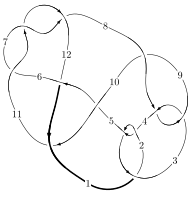
\includegraphics[width=112pt]{../../../GIT/diagram.site/Diagrams/png/943_12a_0142.png}\\
\ \ \ A knot diagram\footnotemark}&
\allowdisplaybreaks
\textbf{Linearized knot diagam} \\
\cline{2-2}
 &
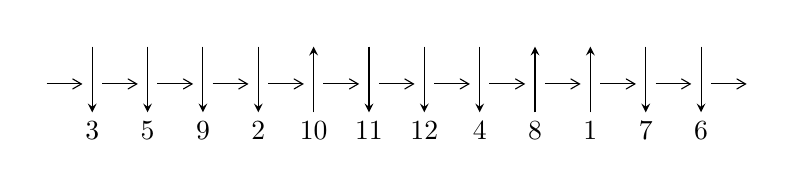
\begin{tikzpicture}[x=20pt, y=17pt]
	% nodes
	\node (C0) at (0, 0) {};
	\node (C1) at (1, 0) {};
	\node (C1U) at (1, +1) {};
	\node (C1D) at (1, -1) {3};

	\node (C2) at (2, 0) {};
	\node (C2U) at (2, +1) {};
	\node (C2D) at (2, -1) {5};

	\node (C3) at (3, 0) {};
	\node (C3U) at (3, +1) {};
	\node (C3D) at (3, -1) {9};

	\node (C4) at (4, 0) {};
	\node (C4U) at (4, +1) {};
	\node (C4D) at (4, -1) {2};

	\node (C5) at (5, 0) {};
	\node (C5U) at (5, +1) {};
	\node (C5D) at (5, -1) {10};

	\node (C6) at (6, 0) {};
	\node (C6U) at (6, +1) {};
	\node (C6D) at (6, -1) {11};

	\node (C7) at (7, 0) {};
	\node (C7U) at (7, +1) {};
	\node (C7D) at (7, -1) {12};

	\node (C8) at (8, 0) {};
	\node (C8U) at (8, +1) {};
	\node (C8D) at (8, -1) {4};

	\node (C9) at (9, 0) {};
	\node (C9U) at (9, +1) {};
	\node (C9D) at (9, -1) {8};

	\node (C10) at (10, 0) {};
	\node (C10U) at (10, +1) {};
	\node (C10D) at (10, -1) {1};

	\node (C11) at (11, 0) {};
	\node (C11U) at (11, +1) {};
	\node (C11D) at (11, -1) {7};

	\node (C12) at (12, 0) {};
	\node (C12U) at (12, +1) {};
	\node (C12D) at (12, -1) {6};
	\node (C13) at (13, 0) {};

	% arrows
	\draw[->,>={angle 60}]
	(C0) edge (C1) (C1) edge (C2) (C2) edge (C3) (C3) edge (C4) (C4) edge (C5) (C5) edge (C6) (C6) edge (C7) (C7) edge (C8) (C8) edge (C9) (C9) edge (C10) (C10) edge (C11) (C11) edge (C12) (C12) edge (C13) ;	\draw[->,>=stealth]
	(C1U) edge (C1D) (C2U) edge (C2D) (C3U) edge (C3D) (C4U) edge (C4D) (C5D) edge (C5U) (C6U) edge (C6D) (C7U) edge (C7D) (C8U) edge (C8D) (C9D) edge (C9U) (C10D) edge (C10U) (C11U) edge (C11D) (C12U) edge (C12D) ;
	\end{tikzpicture} \\
\hhline{~~} \\& 
\textbf{Solving Sequence} \\ \cline{2-2} 
 &
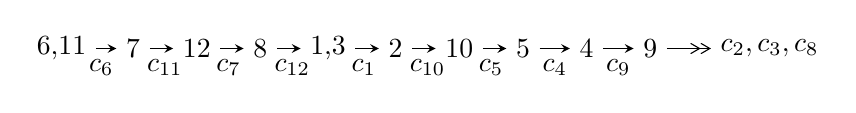
\begin{tikzpicture}[x=23pt, y=7pt]
	% node
	\node (A0) at (-1/8, 0) {6,11};
	\node (A1) at (1, 0) {7};
	\node (A2) at (2, 0) {12};
	\node (A3) at (3, 0) {8};
	\node (A4) at (65/16, 0) {1,3};
	\node (A5) at (41/8, 0) {2};
	\node (A6) at (49/8, 0) {10};
	\node (A7) at (57/8, 0) {5};
	\node (A8) at (65/8, 0) {4};
	\node (A9) at (73/8, 0) {9};
	\node (C1) at (1/2, -1) {$c_{6}$};
	\node (C2) at (3/2, -1) {$c_{11}$};
	\node (C3) at (5/2, -1) {$c_{7}$};
	\node (C4) at (7/2, -1) {$c_{12}$};
	\node (C5) at (37/8, -1) {$c_{1}$};
	\node (C6) at (45/8, -1) {$c_{10}$};
	\node (C7) at (53/8, -1) {$c_{5}$};
	\node (C8) at (61/8, -1) {$c_{4}$};
	\node (C9) at (69/8, -1) {$c_{9}$};
	\node (A10) at (11, 0) {$c_{2},c_{3},c_{8}$};

	% edge
	\draw[->,>=stealth]	
	(A0) edge (A1) (A1) edge (A2) (A2) edge (A3) (A3) edge (A4) (A4) edge (A5) (A5) edge (A6) (A6) edge (A7) (A7) edge (A8) (A8) edge (A9) ;
	\draw[->>,>={angle 60}]	
	(A9) edge (A10);
\end{tikzpicture} \\ 

\end{tabular} \\

\footnotetext{
The image of knot diagram is generated by the software ``\textbf{Draw programme}" developed by Andrew Bartholomew(\url{http://www.layer8.co.uk/maths/draw/index.htm\#Running-draw}), where we modified some parts for our purpose(\url{https://github.com/CATsTAILs/LinksPainter}).
}\phantom \\ \newline 
\centering \textbf{Ideals for irreducible components\footnotemark of $X_{\text{par}}$} 
 
\begin{align*}
I^u_{1}&=\langle 
- u^{96}- u^{95}+\cdots- u^2+b,\;-2 u^{96}-2 u^{95}+\cdots+a-3,\;u^{97}+2 u^{96}+\cdots+u+1\rangle \\
I^u_{2}&=\langle 
b+1,\;u^3+a-2 u,\;u^5+u^4-2 u^3- u^2+u-1\rangle \\
\\
\end{align*}
\raggedright * 2 irreducible components of $\dim_{\mathbb{C}}=0$, with total 102 representations.\\
\footnotetext{All coefficients of polynomials are rational numbers. But the coefficients are sometimes approximated in decimal forms when there is not enough margin.}
\newpage
\renewcommand{\arraystretch}{1}
\centering \section*{I. $I^u_{1}= \langle - u^{96}- u^{95}+\cdots- u^2+b,\;-2 u^{96}-2 u^{95}+\cdots+a-3,\;u^{97}+2 u^{96}+\cdots+u+1 \rangle$}
\flushleft \textbf{(i) Arc colorings}\\
\begin{tabular}{m{7pt} m{180pt} m{7pt} m{180pt} }
\flushright $a_{6}=$&$\begin{pmatrix}1\\0\end{pmatrix}$ \\
\flushright $a_{11}=$&$\begin{pmatrix}0\\u\end{pmatrix}$ \\
\flushright $a_{7}=$&$\begin{pmatrix}1\\u^2\end{pmatrix}$ \\
\flushright $a_{12}=$&$\begin{pmatrix}- u\\- u^3+u\end{pmatrix}$ \\
\flushright $a_{8}=$&$\begin{pmatrix}- u^2+1\\- u^4+2 u^2\end{pmatrix}$ \\
\flushright $a_{1}=$&$\begin{pmatrix}u^3-2 u\\- u^3+u\end{pmatrix}$ \\
\flushright $a_{3}=$&$\begin{pmatrix}2 u^{96}+2 u^{95}+\cdots-2 u^2+3\\u^{96}+u^{95}+\cdots+6 u^3+u^2\end{pmatrix}$ \\
\flushright $a_{2}=$&$\begin{pmatrix}u^{96}+u^{95}+\cdots- u^2+2\\u^{96}+u^{95}+\cdots+2 u^2+u\end{pmatrix}$ \\
\flushright $a_{10}=$&$\begin{pmatrix}- u^7+4 u^5-4 u^3\\u^7-3 u^5+2 u^3+u\end{pmatrix}$ \\
\flushright $a_{5}=$&$\begin{pmatrix}- u^{14}+7 u^{12}-18 u^{10}+19 u^8-4 u^6-4 u^4+1\\u^{14}-6 u^{12}+13 u^{10}-10 u^8-2 u^6+4 u^4+u^2\end{pmatrix}$ \\
\flushright $a_{4}=$&$\begin{pmatrix}u^{83}-38 u^{81}+\cdots-9 u^3+2\\u^{96}+u^{95}+\cdots+3 u^2+u\end{pmatrix}$ \\
\flushright $a_{9}=$&$\begin{pmatrix}- u^{13}+6 u^{11}-13 u^9+10 u^7+2 u^5-4 u^3- u\\- u^{15}+7 u^{13}-18 u^{11}+19 u^9-4 u^7-4 u^5+u\end{pmatrix}$\\&\end{tabular}
\flushleft \textbf{(ii) Obstruction class $= -1$}\\~\\
\flushleft \textbf{(iii) Cusp Shapes $= 6 u^{96}+4 u^{95}+\cdots+5 u-2$}\\~\\
\newpage\renewcommand{\arraystretch}{1}
\flushleft \textbf{(iv) u-Polynomials at the component}\newline \\
\begin{tabular}{m{50pt}|m{274pt}}
Crossings & \hspace{64pt}u-Polynomials at each crossing \\
\hline $$\begin{aligned}c_{1}\end{aligned}$$&$\begin{aligned}
&u^{97}+52 u^{96}+\cdots+7 u+1
\end{aligned}$\\
\hline $$\begin{aligned}c_{2},c_{4}\end{aligned}$$&$\begin{aligned}
&u^{97}-6 u^{96}+\cdots-5 u+1
\end{aligned}$\\
\hline $$\begin{aligned}c_{3},c_{8}\end{aligned}$$&$\begin{aligned}
&u^{97}- u^{96}+\cdots+32 u+32
\end{aligned}$\\
\hline $$\begin{aligned}c_{5}\end{aligned}$$&$\begin{aligned}
&u^{97}-2 u^{96}+\cdots-939 u+137
\end{aligned}$\\
\hline $$\begin{aligned}c_{6},c_{7},c_{11}\end{aligned}$$&$\begin{aligned}
&u^{97}+2 u^{96}+\cdots+u+1
\end{aligned}$\\
\hline $$\begin{aligned}c_{9}\end{aligned}$$&$\begin{aligned}
&u^{97}-33 u^{96}+\cdots-22016 u+1024
\end{aligned}$\\
\hline $$\begin{aligned}c_{10}\end{aligned}$$&$\begin{aligned}
&u^{97}+20 u^{96}+\cdots+152213 u+6497
\end{aligned}$\\
\hline $$\begin{aligned}c_{12}\end{aligned}$$&$\begin{aligned}
&u^{97}-6 u^{96}+\cdots-63 u+5
\end{aligned}$\\
\hline
\end{tabular}\\~\\
\newpage\renewcommand{\arraystretch}{1}
\flushleft \textbf{(v) Riley Polynomials at the component}\newline \\
\begin{tabular}{m{50pt}|m{274pt}}
Crossings & \hspace{64pt}Riley Polynomials at each crossing \\
\hline $$\begin{aligned}c_{1}\end{aligned}$$&$\begin{aligned}
&y^{97}-8 y^{96}+\cdots+23 y-1
\end{aligned}$\\
\hline $$\begin{aligned}c_{2},c_{4}\end{aligned}$$&$\begin{aligned}
&y^{97}-52 y^{96}+\cdots+7 y-1
\end{aligned}$\\
\hline $$\begin{aligned}c_{3},c_{8}\end{aligned}$$&$\begin{aligned}
&y^{97}+33 y^{96}+\cdots-22016 y-1024
\end{aligned}$\\
\hline $$\begin{aligned}c_{5}\end{aligned}$$&$\begin{aligned}
&y^{97}+86 y^{95}+\cdots+940357 y-18769
\end{aligned}$\\
\hline $$\begin{aligned}c_{6},c_{7},c_{11}\end{aligned}$$&$\begin{aligned}
&y^{97}-88 y^{96}+\cdots+5 y-1
\end{aligned}$\\
\hline $$\begin{aligned}c_{9}\end{aligned}$$&$\begin{aligned}
&y^{97}+53 y^{96}+\cdots+30015488 y-1048576
\end{aligned}$\\
\hline $$\begin{aligned}c_{10}\end{aligned}$$&$\begin{aligned}
&y^{97}+36 y^{96}+\cdots+514538009 y-42211009
\end{aligned}$\\
\hline $$\begin{aligned}c_{12}\end{aligned}$$&$\begin{aligned}
&y^{97}-8 y^{96}+\cdots+569 y-25
\end{aligned}$\\
\hline
\end{tabular}\\~\\
\newpage\flushleft \textbf{(vi) Complex Volumes and Cusp Shapes}
$$\begin{array}{c|c|c}  
\text{Solutions to }I^u_{1}& \I (\text{vol} + \sqrt{-1}CS) & \text{Cusp shape}\\
 \hline 
\begin{aligned}
u &= \phantom{-}0.943941 + 0.121484 I \\
a &= -0.496423 - 0.405418 I \\
b &= \phantom{-}0.061982 - 0.953000 I\end{aligned}
 & \phantom{-}2.92060 - 2.48348 I & \phantom{-0.000000 } 0 \\ \hline\begin{aligned}
u &= \phantom{-}0.943941 - 0.121484 I \\
a &= -0.496423 + 0.405418 I \\
b &= \phantom{-}0.061982 + 0.953000 I\end{aligned}
 & \phantom{-}2.92060 + 2.48348 I & \phantom{-0.000000 } 0 \\ \hline\begin{aligned}
u &= \phantom{-}1.111500 + 0.195710 I \\
a &= -0.991198 + 0.480915 I \\
b &= \phantom{-}0.157594 + 0.050205 I\end{aligned}
 & \phantom{-}0.42510 - 4.54620 I & \phantom{-0.000000 } 0 \\ \hline\begin{aligned}
u &= \phantom{-}1.111500 - 0.195710 I \\
a &= -0.991198 - 0.480915 I \\
b &= \phantom{-}0.157594 - 0.050205 I\end{aligned}
 & \phantom{-}0.42510 + 4.54620 I & \phantom{-0.000000 } 0 \\ \hline\begin{aligned}
u &= -1.132700 + 0.052850 I \\
a &= \phantom{-}0.910466 + 0.414617 I \\
b &= \phantom{-}0.450519 + 0.261516 I\end{aligned}
 & -1.77925 + 0.16252 I & \phantom{-0.000000 } 0 \\ \hline\begin{aligned}
u &= -1.132700 - 0.052850 I \\
a &= \phantom{-}0.910466 - 0.414617 I \\
b &= \phantom{-}0.450519 - 0.261516 I\end{aligned}
 & -1.77925 - 0.16252 I & \phantom{-0.000000 } 0 \\ \hline\begin{aligned}
u &= \phantom{-}1.134230 + 0.229902 I \\
a &= \phantom{-}0.951922 - 0.710835 I \\
b &= -0.076764 - 0.808674 I\end{aligned}
 & -2.13303 - 9.58468 I & \phantom{-0.000000 } 0 \\ \hline\begin{aligned}
u &= \phantom{-}1.134230 - 0.229902 I \\
a &= \phantom{-}0.951922 + 0.710835 I \\
b &= -0.076764 + 0.808674 I\end{aligned}
 & -2.13303 + 9.58468 I & \phantom{-0.000000 } 0 \\ \hline\begin{aligned}
u &= -1.145920 + 0.167609 I \\
a &= -0.559216 - 1.229480 I \\
b &= -0.169401 - 1.056630 I\end{aligned}
 & -3.77103 + 3.82064 I & \phantom{-0.000000 } 0 \\ \hline\begin{aligned}
u &= -1.145920 - 0.167609 I \\
a &= -0.559216 + 1.229480 I \\
b &= -0.169401 + 1.056630 I\end{aligned}
 & -3.77103 - 3.82064 I & \phantom{-0.000000 } 0\\
 \hline 
 \end{array}$$\newpage$$\begin{array}{c|c|c}  
\text{Solutions to }I^u_{1}& \I (\text{vol} + \sqrt{-1}CS) & \text{Cusp shape}\\
 \hline 
\begin{aligned}
u &= \phantom{-}1.168790 + 0.130280 I \\
a &= \phantom{-}0.892219 - 0.513776 I \\
b &= -1.193000 + 0.490171 I\end{aligned}
 & -4.25351 - 1.40778 I & \phantom{-0.000000 } 0 \\ \hline\begin{aligned}
u &= \phantom{-}1.168790 - 0.130280 I \\
a &= \phantom{-}0.892219 + 0.513776 I \\
b &= -1.193000 - 0.490171 I\end{aligned}
 & -4.25351 + 1.40778 I & \phantom{-0.000000 } 0 \\ \hline\begin{aligned}
u &= \phantom{-}0.312759 + 0.712439 I \\
a &= \phantom{-}2.39656 + 3.11419 I \\
b &= -2.56647 - 1.59551 I\end{aligned}
 & -1.81149 - 13.02420 I & -6.49881 + 10.34514 I \\ \hline\begin{aligned}
u &= \phantom{-}0.312759 - 0.712439 I \\
a &= \phantom{-}2.39656 - 3.11419 I \\
b &= -2.56647 + 1.59551 I\end{aligned}
 & -1.81149 + 13.02420 I & -6.49881 - 10.34514 I \\ \hline\begin{aligned}
u &= \phantom{-}0.300843 + 0.702322 I \\
a &= -1.91199 - 2.03390 I \\
b &= \phantom{-}1.65378 + 0.88080 I\end{aligned}
 & \phantom{-}1.08712 - 7.85100 I & -3.11991 + 7.31455 I \\ \hline\begin{aligned}
u &= \phantom{-}0.300843 - 0.702322 I \\
a &= -1.91199 + 2.03390 I \\
b &= \phantom{-}1.65378 - 0.88080 I\end{aligned}
 & \phantom{-}1.08712 + 7.85100 I & -3.11991 - 7.31455 I \\ \hline\begin{aligned}
u &= -0.308505 + 0.689688 I \\
a &= -3.08907 + 2.22676 I \\
b &= \phantom{-}2.80515 - 0.95593 I\end{aligned}
 & -3.16701 + 6.77469 I & -8.01279 - 6.91414 I \\ \hline\begin{aligned}
u &= -0.308505 - 0.689688 I \\
a &= -3.08907 - 2.22676 I \\
b &= \phantom{-}2.80515 + 0.95593 I\end{aligned}
 & -3.16701 - 6.77469 I & -8.01279 + 6.91414 I \\ \hline\begin{aligned}
u &= \phantom{-}0.623987 + 0.420887 I \\
a &= \phantom{-}2.44137 + 1.67780 I \\
b &= -1.90511 + 0.66513 I\end{aligned}
 & -3.01492 + 9.05165 I & -8.99353 - 5.05015 I \\ \hline\begin{aligned}
u &= \phantom{-}0.623987 - 0.420887 I \\
a &= \phantom{-}2.44137 - 1.67780 I \\
b &= -1.90511 - 0.66513 I\end{aligned}
 & -3.01492 - 9.05165 I & -8.99353 + 5.05015 I\\
 \hline 
 \end{array}$$\newpage$$\begin{array}{c|c|c}  
\text{Solutions to }I^u_{1}& \I (\text{vol} + \sqrt{-1}CS) & \text{Cusp shape}\\
 \hline 
\begin{aligned}
u &= -0.353257 + 0.664610 I \\
a &= -2.80675 - 0.31529 I \\
b &= \phantom{-}1.59380 + 1.22211 I\end{aligned}
 & -3.61011 - 0.93729 I & -8.61161 + 0.95257 I \\ \hline\begin{aligned}
u &= -0.353257 - 0.664610 I \\
a &= -2.80675 + 0.31529 I \\
b &= \phantom{-}1.59380 - 1.22211 I\end{aligned}
 & -3.61011 + 0.93729 I & -8.61161 - 0.95257 I \\ \hline\begin{aligned}
u &= \phantom{-}0.729778 + 0.164872 I \\
a &= -0.173384 + 0.743443 I \\
b &= -0.170411 + 0.615315 I\end{aligned}
 & \phantom{-}2.85417 + 2.45539 I & -3.14691 - 2.99420 I \\ \hline\begin{aligned}
u &= \phantom{-}0.729778 - 0.164872 I \\
a &= -0.173384 - 0.743443 I \\
b &= -0.170411 - 0.615315 I\end{aligned}
 & \phantom{-}2.85417 - 2.45539 I & -3.14691 + 2.99420 I \\ \hline\begin{aligned}
u &= \phantom{-}0.311458 + 0.677389 I \\
a &= \phantom{-}3.11096 + 0.73852 I \\
b &= -2.00323 + 0.70708 I\end{aligned}
 & -3.56160 - 4.04042 I & -8.16281 + 6.14210 I \\ \hline\begin{aligned}
u &= \phantom{-}0.311458 - 0.677389 I \\
a &= \phantom{-}3.11096 - 0.73852 I \\
b &= -2.00323 - 0.70708 I\end{aligned}
 & -3.56160 + 4.04042 I & -8.16281 - 6.14210 I \\ \hline\begin{aligned}
u &= \phantom{-}0.234210 + 0.696927 I \\
a &= \phantom{-}0.505572 + 0.362097 I \\
b &= -0.947702 - 0.309326 I\end{aligned}
 & \phantom{-}4.69343 - 5.97822 I & -0.22935 + 7.86187 I \\ \hline\begin{aligned}
u &= \phantom{-}0.234210 - 0.696927 I \\
a &= \phantom{-}0.505572 - 0.362097 I \\
b &= -0.947702 + 0.309326 I\end{aligned}
 & \phantom{-}4.69343 + 5.97822 I & -0.22935 - 7.86187 I \\ \hline\begin{aligned}
u &= -0.302548 + 0.652337 I \\
a &= \phantom{-}1.69438 - 1.39167 I \\
b &= -1.276750 + 0.594963 I\end{aligned}
 & -0.47477 + 2.56834 I & -4.93539 - 3.16377 I \\ \hline\begin{aligned}
u &= -0.302548 - 0.652337 I \\
a &= \phantom{-}1.69438 + 1.39167 I \\
b &= -1.276750 - 0.594963 I\end{aligned}
 & -0.47477 - 2.56834 I & -4.93539 + 3.16377 I\\
 \hline 
 \end{array}$$\newpage$$\begin{array}{c|c|c}  
\text{Solutions to }I^u_{1}& \I (\text{vol} + \sqrt{-1}CS) & \text{Cusp shape}\\
 \hline 
\begin{aligned}
u &= \phantom{-}0.607220 + 0.381444 I \\
a &= -1.51037 - 1.12452 I \\
b &= \phantom{-}1.240080 - 0.073557 I\end{aligned}
 & -0.15886 + 4.01632 I & -5.76175 - 1.99933 I \\ \hline\begin{aligned}
u &= \phantom{-}0.607220 - 0.381444 I \\
a &= -1.51037 + 1.12452 I \\
b &= \phantom{-}1.240080 + 0.073557 I\end{aligned}
 & -0.15886 - 4.01632 I & -5.76175 + 1.99933 I \\ \hline\begin{aligned}
u &= -0.520379 + 0.490382 I \\
a &= \phantom{-}0.35702 + 2.38031 I \\
b &= \phantom{-}1.09071 - 1.54215 I\end{aligned}
 & -4.31532 + 4.81391 I & -10.30909 - 7.09591 I \\ \hline\begin{aligned}
u &= -0.520379 - 0.490382 I \\
a &= \phantom{-}0.35702 - 2.38031 I \\
b &= \phantom{-}1.09071 + 1.54215 I\end{aligned}
 & -4.31532 - 4.81391 I & -10.30909 + 7.09591 I \\ \hline\begin{aligned}
u &= \phantom{-}0.198968 + 0.686527 I \\
a &= -0.629727 - 1.247650 I \\
b &= \phantom{-}0.923922 + 0.937313 I\end{aligned}
 & \phantom{-}5.13223 - 0.90715 I & \phantom{-}1.37210 + 1.29920 I \\ \hline\begin{aligned}
u &= \phantom{-}0.198968 - 0.686527 I \\
a &= -0.629727 + 1.247650 I \\
b &= \phantom{-}0.923922 - 0.937313 I\end{aligned}
 & \phantom{-}5.13223 + 0.90715 I & \phantom{-}1.37210 - 1.29920 I \\ \hline\begin{aligned}
u &= -1.278380 + 0.233147 I \\
a &= -0.144124 - 0.663246 I \\
b &= \phantom{-}0.813649 + 0.516215 I\end{aligned}
 & -3.08467 - 2.82936 I & \phantom{-0.000000 } 0 \\ \hline\begin{aligned}
u &= -1.278380 - 0.233147 I \\
a &= -0.144124 + 0.663246 I \\
b &= \phantom{-}0.813649 - 0.516215 I\end{aligned}
 & -3.08467 + 2.82936 I & \phantom{-0.000000 } 0 \\ \hline\begin{aligned}
u &= -0.567881 + 0.398456 I \\
a &= -1.90800 + 2.59584 I \\
b &= \phantom{-}1.73968 - 0.00180 I\end{aligned}
 & -4.28231 - 2.99360 I & -10.93115 + 1.06271 I \\ \hline\begin{aligned}
u &= -0.567881 - 0.398456 I \\
a &= -1.90800 - 2.59584 I \\
b &= \phantom{-}1.73968 + 0.00180 I\end{aligned}
 & -4.28231 + 2.99360 I & -10.93115 - 1.06271 I\\
 \hline 
 \end{array}$$\newpage$$\begin{array}{c|c|c}  
\text{Solutions to }I^u_{1}& \I (\text{vol} + \sqrt{-1}CS) & \text{Cusp shape}\\
 \hline 
\begin{aligned}
u &= \phantom{-}0.068167 + 0.685266 I \\
a &= \phantom{-}0.172272 + 1.080270 I \\
b &= \phantom{-}0.519079 + 0.016412 I\end{aligned}
 & \phantom{-}1.06783 + 6.16150 I & -2.45385 - 4.75788 I \\ \hline\begin{aligned}
u &= \phantom{-}0.068167 - 0.685266 I \\
a &= \phantom{-}0.172272 - 1.080270 I \\
b &= \phantom{-}0.519079 - 0.016412 I\end{aligned}
 & \phantom{-}1.06783 - 6.16150 I & -2.45385 + 4.75788 I \\ \hline\begin{aligned}
u &= -0.375160 + 0.561170 I \\
a &= \phantom{-}0.268255 + 0.166885 I \\
b &= \phantom{-}0.1081490 + 0.0316957 I\end{aligned}
 & -1.03389 + 1.75402 I & -2.33100 - 5.04441 I \\ \hline\begin{aligned}
u &= -0.375160 - 0.561170 I \\
a &= \phantom{-}0.268255 - 0.166885 I \\
b &= \phantom{-}0.1081490 - 0.0316957 I\end{aligned}
 & -1.03389 - 1.75402 I & -2.33100 + 5.04441 I \\ \hline\begin{aligned}
u &= \phantom{-}0.535382 + 0.408739 I \\
a &= \phantom{-}0.20878 + 2.11033 I \\
b &= -1.56265 - 1.13569 I\end{aligned}
 & -4.57857 + 0.32685 I & -11.21882 + 0.05170 I \\ \hline\begin{aligned}
u &= \phantom{-}0.535382 - 0.408739 I \\
a &= \phantom{-}0.20878 - 2.11033 I \\
b &= -1.56265 + 1.13569 I\end{aligned}
 & -4.57857 - 0.32685 I & -11.21882 - 0.05170 I \\ \hline\begin{aligned}
u &= \phantom{-}0.105616 + 0.661702 I \\
a &= -0.41822 - 1.42393 I \\
b &= \phantom{-}0.045797 + 0.498373 I\end{aligned}
 & \phantom{-}3.40166 + 1.28266 I & \phantom{-}1.322307 - 0.278436 I \\ \hline\begin{aligned}
u &= \phantom{-}0.105616 - 0.661702 I \\
a &= -0.41822 + 1.42393 I \\
b &= \phantom{-}0.045797 - 0.498373 I\end{aligned}
 & \phantom{-}3.40166 - 1.28266 I & \phantom{-}1.322307 + 0.278436 I \\ \hline\begin{aligned}
u &= -0.217493 + 0.618562 I \\
a &= -0.39149 - 1.70038 I \\
b &= \phantom{-}0.474158 + 1.007980 I\end{aligned}
 & \phantom{-}0.49581 + 2.43913 I & -3.27691 - 6.47368 I \\ \hline\begin{aligned}
u &= -0.217493 - 0.618562 I \\
a &= -0.39149 + 1.70038 I \\
b &= \phantom{-}0.474158 - 1.007980 I\end{aligned}
 & \phantom{-}0.49581 - 2.43913 I & -3.27691 + 6.47368 I\\
 \hline 
 \end{array}$$\newpage$$\begin{array}{c|c|c}  
\text{Solutions to }I^u_{1}& \I (\text{vol} + \sqrt{-1}CS) & \text{Cusp shape}\\
 \hline 
\begin{aligned}
u &= -1.326350 + 0.232749 I \\
a &= \phantom{-}0.341783 + 0.812780 I \\
b &= \phantom{-}0.219491 - 0.801362 I\end{aligned}
 & -1.07006 + 1.93167 I & \phantom{-0.000000 } 0 \\ \hline\begin{aligned}
u &= -1.326350 - 0.232749 I \\
a &= \phantom{-}0.341783 - 0.812780 I \\
b &= \phantom{-}0.219491 + 0.801362 I\end{aligned}
 & -1.07006 - 1.93167 I & \phantom{-0.000000 } 0 \\ \hline\begin{aligned}
u &= -1.365960 + 0.054249 I \\
a &= -0.218600 - 0.681410 I \\
b &= \phantom{-}0.273700 + 0.033467 I\end{aligned}
 & -3.12013 - 1.90937 I & \phantom{-0.000000 } 0 \\ \hline\begin{aligned}
u &= -1.365960 - 0.054249 I \\
a &= -0.218600 + 0.681410 I \\
b &= \phantom{-}0.273700 - 0.033467 I\end{aligned}
 & -3.12013 + 1.90937 I & \phantom{-0.000000 } 0 \\ \hline\begin{aligned}
u &= -0.467096 + 0.419960 I \\
a &= \phantom{-}0.90569 - 1.35055 I \\
b &= -0.820519 + 0.455130 I\end{aligned}
 & -1.34526 + 0.92967 I & -7.49316 - 3.69890 I \\ \hline\begin{aligned}
u &= -0.467096 - 0.419960 I \\
a &= \phantom{-}0.90569 + 1.35055 I \\
b &= -0.820519 - 0.455130 I\end{aligned}
 & -1.34526 - 0.92967 I & -7.49316 + 3.69890 I \\ \hline\begin{aligned}
u &= \phantom{-}1.361400 + 0.206058 I \\
a &= \phantom{-}0.723724 + 0.180323 I \\
b &= -1.75482 + 0.80199 I\end{aligned}
 & -5.27906 - 1.90423 I & \phantom{-0.000000 } 0 \\ \hline\begin{aligned}
u &= \phantom{-}1.361400 - 0.206058 I \\
a &= \phantom{-}0.723724 - 0.180323 I \\
b &= -1.75482 - 0.80199 I\end{aligned}
 & -5.27906 + 1.90423 I & \phantom{-0.000000 } 0 \\ \hline\begin{aligned}
u &= -0.089375 + 0.596895 I \\
a &= \phantom{-}1.24278 + 1.08334 I \\
b &= -1.095750 + 0.055567 I\end{aligned}
 & -0.654118 - 0.881098 I & -4.24003 + 0.39048 I \\ \hline\begin{aligned}
u &= -0.089375 - 0.596895 I \\
a &= \phantom{-}1.24278 - 1.08334 I \\
b &= -1.095750 - 0.055567 I\end{aligned}
 & -0.654118 + 0.881098 I & -4.24003 - 0.39048 I\\
 \hline 
 \end{array}$$\newpage$$\begin{array}{c|c|c}  
\text{Solutions to }I^u_{1}& \I (\text{vol} + \sqrt{-1}CS) & \text{Cusp shape}\\
 \hline 
\begin{aligned}
u &= -1.373470 + 0.266918 I \\
a &= \phantom{-}0.479744 + 0.763399 I \\
b &= \phantom{-}1.43196 - 0.71930 I\end{aligned}
 & \phantom{-}0.14596 + 4.36125 I & \phantom{-0.000000 } 0 \\ \hline\begin{aligned}
u &= -1.373470 - 0.266918 I \\
a &= \phantom{-}0.479744 - 0.763399 I \\
b &= \phantom{-}1.43196 + 0.71930 I\end{aligned}
 & \phantom{-}0.14596 - 4.36125 I & \phantom{-0.000000 } 0 \\ \hline\begin{aligned}
u &= -1.383370 + 0.219886 I \\
a &= -0.61670 - 1.52897 I \\
b &= -1.54081 + 0.33905 I\end{aligned}
 & -6.34678 + 3.87671 I & \phantom{-0.000000 } 0 \\ \hline\begin{aligned}
u &= -1.383370 - 0.219886 I \\
a &= -0.61670 + 1.52897 I \\
b &= -1.54081 - 0.33905 I\end{aligned}
 & -6.34678 - 3.87671 I & \phantom{-0.000000 } 0 \\ \hline\begin{aligned}
u &= \phantom{-}1.385740 + 0.240581 I \\
a &= -0.777813 + 0.354416 I \\
b &= \phantom{-}0.50379 - 1.82800 I\end{aligned}
 & -4.61803 - 5.57776 I & \phantom{-0.000000 } 0 \\ \hline\begin{aligned}
u &= \phantom{-}1.385740 - 0.240581 I \\
a &= -0.777813 - 0.354416 I \\
b &= \phantom{-}0.50379 + 1.82800 I\end{aligned}
 & -4.61803 + 5.57776 I & \phantom{-0.000000 } 0 \\ \hline\begin{aligned}
u &= -1.39052 + 0.27429 I \\
a &= -0.183283 - 0.415905 I \\
b &= -1.247440 - 0.130862 I\end{aligned}
 & -0.47363 + 9.50479 I & \phantom{-0.000000 } 0 \\ \hline\begin{aligned}
u &= -1.39052 - 0.27429 I \\
a &= -0.183283 + 0.415905 I \\
b &= -1.247440 + 0.130862 I\end{aligned}
 & -0.47363 - 9.50479 I & \phantom{-0.000000 } 0 \\ \hline\begin{aligned}
u &= \phantom{-}0.187132 + 0.543748 I \\
a &= \phantom{-}1.14094 + 2.10115 I \\
b &= -1.284210 - 0.281999 I\end{aligned}
 & -1.29274 - 1.03812 I & -1.55594 - 0.13944 I \\ \hline\begin{aligned}
u &= \phantom{-}0.187132 - 0.543748 I \\
a &= \phantom{-}1.14094 - 2.10115 I \\
b &= -1.284210 + 0.281999 I\end{aligned}
 & -1.29274 + 1.03812 I & -1.55594 + 0.13944 I\\
 \hline 
 \end{array}$$\newpage$$\begin{array}{c|c|c}  
\text{Solutions to }I^u_{1}& \I (\text{vol} + \sqrt{-1}CS) & \text{Cusp shape}\\
 \hline 
\begin{aligned}
u &= \phantom{-}1.43202 + 0.16090 I \\
a &= -0.448090 + 0.955833 I \\
b &= -1.47938 - 1.33154 I\end{aligned}
 & -7.33738 - 3.08646 I & \phantom{-0.000000 } 0 \\ \hline\begin{aligned}
u &= \phantom{-}1.43202 - 0.16090 I \\
a &= -0.448090 - 0.955833 I \\
b &= -1.47938 + 1.33154 I\end{aligned}
 & -7.33738 + 3.08646 I & \phantom{-0.000000 } 0 \\ \hline\begin{aligned}
u &= \phantom{-}1.41933 + 0.25558 I \\
a &= -0.012553 + 1.400220 I \\
b &= -2.01561 - 0.87988 I\end{aligned}
 & -5.98214 - 5.89543 I & \phantom{-0.000000 } 0 \\ \hline\begin{aligned}
u &= \phantom{-}1.41933 - 0.25558 I \\
a &= -0.012553 - 1.400220 I \\
b &= -2.01561 + 0.87988 I\end{aligned}
 & -5.98214 + 5.89543 I & \phantom{-0.000000 } 0 \\ \hline\begin{aligned}
u &= -1.43824 + 0.12743 I \\
a &= \phantom{-}0.263451 + 1.016370 I \\
b &= \phantom{-}1.92173 - 0.86852 I\end{aligned}
 & -6.50701 - 2.29026 I & \phantom{-0.000000 } 0 \\ \hline\begin{aligned}
u &= -1.43824 - 0.12743 I \\
a &= \phantom{-}0.263451 - 1.016370 I \\
b &= \phantom{-}1.92173 + 0.86852 I\end{aligned}
 & -6.50701 + 2.29026 I & \phantom{-0.000000 } 0 \\ \hline\begin{aligned}
u &= -1.43864 + 0.14807 I \\
a &= -1.32009 - 0.89318 I \\
b &= -1.84164 + 1.95956 I\end{aligned}
 & -10.76520 + 1.67811 I & \phantom{-0.000000 } 0 \\ \hline\begin{aligned}
u &= -1.43864 - 0.14807 I \\
a &= -1.32009 + 0.89318 I \\
b &= -1.84164 - 1.95956 I\end{aligned}
 & -10.76520 - 1.67811 I & \phantom{-0.000000 } 0 \\ \hline\begin{aligned}
u &= \phantom{-}1.43979 + 0.13950 I \\
a &= \phantom{-}0.44600 - 1.88435 I \\
b &= \phantom{-}2.30164 + 1.55417 I\end{aligned}
 & -10.55100 + 1.09910 I & \phantom{-0.000000 } 0 \\ \hline\begin{aligned}
u &= \phantom{-}1.43979 - 0.13950 I \\
a &= \phantom{-}0.44600 + 1.88435 I \\
b &= \phantom{-}2.30164 - 1.55417 I\end{aligned}
 & -10.55100 - 1.09910 I & \phantom{-0.000000 } 0\\
 \hline 
 \end{array}$$\newpage$$\begin{array}{c|c|c}  
\text{Solutions to }I^u_{1}& \I (\text{vol} + \sqrt{-1}CS) & \text{Cusp shape}\\
 \hline 
\begin{aligned}
u &= -1.42444 + 0.26341 I \\
a &= \phantom{-}0.92067 - 1.92713 I \\
b &= -2.38606 - 0.59877 I\end{aligned}
 & -9.11571 + 7.47577 I & \phantom{-0.000000 } 0 \\ \hline\begin{aligned}
u &= -1.42444 - 0.26341 I \\
a &= \phantom{-}0.92067 + 1.92713 I \\
b &= -2.38606 + 0.59877 I\end{aligned}
 & -9.11571 - 7.47577 I & \phantom{-0.000000 } 0 \\ \hline\begin{aligned}
u &= -1.42255 + 0.27432 I \\
a &= \phantom{-}0.21487 + 1.75795 I \\
b &= \phantom{-}2.20011 - 1.19121 I\end{aligned}
 & -4.42341 + 11.40850 I & \phantom{-0.000000 } 0 \\ \hline\begin{aligned}
u &= -1.42255 - 0.27432 I \\
a &= \phantom{-}0.21487 - 1.75795 I \\
b &= \phantom{-}2.20011 + 1.19121 I\end{aligned}
 & -4.42341 - 11.40850 I & \phantom{-0.000000 } 0 \\ \hline\begin{aligned}
u &= \phantom{-}1.42451 + 0.26845 I \\
a &= \phantom{-}0.02143 - 2.31717 I \\
b &= \phantom{-}3.74912 + 1.01151 I\end{aligned}
 & -8.71124 - 10.26900 I & \phantom{-0.000000 } 0 \\ \hline\begin{aligned}
u &= \phantom{-}1.42451 - 0.26845 I \\
a &= \phantom{-}0.02143 + 2.31717 I \\
b &= \phantom{-}3.74912 - 1.01151 I\end{aligned}
 & -8.71124 + 10.26900 I & \phantom{-0.000000 } 0 \\ \hline\begin{aligned}
u &= \phantom{-}1.43397 + 0.21556 I \\
a &= \phantom{-}0.232723 - 0.151810 I \\
b &= \phantom{-}0.0590316 - 0.0776960 I\end{aligned}
 & -6.82096 - 4.62626 I & \phantom{-0.000000 } 0 \\ \hline\begin{aligned}
u &= \phantom{-}1.43397 - 0.21556 I \\
a &= \phantom{-}0.232723 + 0.151810 I \\
b &= \phantom{-}0.0590316 + 0.0776960 I\end{aligned}
 & -6.82096 + 4.62626 I & \phantom{-0.000000 } 0 \\ \hline\begin{aligned}
u &= -1.42861 + 0.27754 I \\
a &= -0.65259 - 2.39504 I \\
b &= -3.29315 + 1.85894 I\end{aligned}
 & -7.3834 + 16.6288 I & \phantom{-0.000000 } 0 \\ \hline\begin{aligned}
u &= -1.42861 - 0.27754 I \\
a &= -0.65259 + 2.39504 I \\
b &= -3.29315 - 1.85894 I\end{aligned}
 & -7.3834 - 16.6288 I & \phantom{-0.000000 } 0\\
 \hline 
 \end{array}$$\newpage$$\begin{array}{c|c|c}  
\text{Solutions to }I^u_{1}& \I (\text{vol} + \sqrt{-1}CS) & \text{Cusp shape}\\
 \hline 
\begin{aligned}
u &= -1.45265 + 0.12554 I \\
a &= -0.02515 - 1.78570 I \\
b &= -2.63824 + 0.60627 I\end{aligned}
 & -9.55042 - 7.23704 I & \phantom{-0.000000 } 0 \\ \hline\begin{aligned}
u &= -1.45265 - 0.12554 I \\
a &= -0.02515 + 1.78570 I \\
b &= -2.63824 - 0.60627 I\end{aligned}
 & -9.55042 + 7.23704 I & \phantom{-0.000000 } 0 \\ \hline\begin{aligned}
u &= \phantom{-}1.43834 + 0.25272 I \\
a &= -1.21346 - 1.31458 I \\
b &= \phantom{-}2.01713 - 1.23238 I\end{aligned}
 & -9.35467 - 2.41231 I & \phantom{-0.000000 } 0 \\ \hline\begin{aligned}
u &= \phantom{-}1.43834 - 0.25272 I \\
a &= -1.21346 + 1.31458 I \\
b &= \phantom{-}2.01713 + 1.23238 I\end{aligned}
 & -9.35467 + 2.41231 I & \phantom{-0.000000 } 0 \\ \hline\begin{aligned}
u &= \phantom{-}1.45325 + 0.16584 I \\
a &= \phantom{-}1.40656 - 0.73172 I \\
b &= \phantom{-}1.09821 + 2.30833 I\end{aligned}
 & -10.60000 - 7.15506 I & \phantom{-0.000000 } 0 \\ \hline\begin{aligned}
u &= \phantom{-}1.45325 - 0.16584 I \\
a &= \phantom{-}1.40656 + 0.73172 I \\
b &= \phantom{-}1.09821 - 2.30833 I\end{aligned}
 & -10.60000 + 7.15506 I & \phantom{-0.000000 } 0 \\ \hline\begin{aligned}
u &= -0.317685\phantom{ +0.000000I} \\
a &= \phantom{-}2.49633\phantom{ +0.000000I} \\
b &= -0.369663\phantom{ +0.000000I}\end{aligned}
 & -1.03010\phantom{ +0.000000I} & -10.3530\phantom{ +0.000000I}\\
 \hline 
 \end{array}$$\newpage\newpage\renewcommand{\arraystretch}{1}
\centering \section*{II. $I^u_{2}= \langle b+1,\;u^3+a-2 u,\;u^5+u^4-2 u^3- u^2+u-1 \rangle$}
\flushleft \textbf{(i) Arc colorings}\\
\begin{tabular}{m{7pt} m{180pt} m{7pt} m{180pt} }
\flushright $a_{6}=$&$\begin{pmatrix}1\\0\end{pmatrix}$ \\
\flushright $a_{11}=$&$\begin{pmatrix}0\\u\end{pmatrix}$ \\
\flushright $a_{7}=$&$\begin{pmatrix}1\\u^2\end{pmatrix}$ \\
\flushright $a_{12}=$&$\begin{pmatrix}- u\\- u^3+u\end{pmatrix}$ \\
\flushright $a_{8}=$&$\begin{pmatrix}- u^2+1\\- u^4+2 u^2\end{pmatrix}$ \\
\flushright $a_{1}=$&$\begin{pmatrix}u^3-2 u\\- u^3+u\end{pmatrix}$ \\
\flushright $a_{3}=$&$\begin{pmatrix}- u^3+2 u\\-1\end{pmatrix}$ \\
\flushright $a_{2}=$&$\begin{pmatrix}0\\- u^3+u-1\end{pmatrix}$ \\
\flushright $a_{10}=$&$\begin{pmatrix}- u^2+1\\- u^4+2 u^2\end{pmatrix}$ \\
\flushright $a_{5}=$&$\begin{pmatrix}- u^3+2 u\\u^3- u\end{pmatrix}$ \\
\flushright $a_{4}=$&$\begin{pmatrix}- u^3+2 u\\-1\end{pmatrix}$ \\
\flushright $a_{9}=$&$\begin{pmatrix}- u^2+1\\- u^4+2 u^2\end{pmatrix}$\\&\end{tabular}
\flushleft \textbf{(ii) Obstruction class $= 1$}\\~\\
\flushleft \textbf{(iii) Cusp Shapes $= -3 u^3+u^2+8 u-15$}\\~\\
\newpage\renewcommand{\arraystretch}{1}
\flushleft \textbf{(iv) u-Polynomials at the component}\newline \\
\begin{tabular}{m{50pt}|m{274pt}}
Crossings & \hspace{64pt}u-Polynomials at each crossing \\
\hline $$\begin{aligned}c_{1},c_{2}\end{aligned}$$&$\begin{aligned}
&(u-1)^5
\end{aligned}$\\
\hline $$\begin{aligned}c_{3},c_{8},c_{9}\end{aligned}$$&$\begin{aligned}
&u^5
\end{aligned}$\\
\hline $$\begin{aligned}c_{4}\end{aligned}$$&$\begin{aligned}
&(u+1)^5
\end{aligned}$\\
\hline $$\begin{aligned}c_{5},c_{10}\end{aligned}$$&$\begin{aligned}
&u^5- u^4+2 u^3- u^2+u-1
\end{aligned}$\\
\hline $$\begin{aligned}c_{6},c_{7}\end{aligned}$$&$\begin{aligned}
&u^5+u^4-2 u^3- u^2+u-1
\end{aligned}$\\
\hline $$\begin{aligned}c_{11}\end{aligned}$$&$\begin{aligned}
&u^5- u^4-2 u^3+u^2+u+1
\end{aligned}$\\
\hline $$\begin{aligned}c_{12}\end{aligned}$$&$\begin{aligned}
&u^5+3 u^4+4 u^3+u^2- u-1
\end{aligned}$\\
\hline
\end{tabular}\\~\\
\newpage\renewcommand{\arraystretch}{1}
\flushleft \textbf{(v) Riley Polynomials at the component}\newline \\
\begin{tabular}{m{50pt}|m{274pt}}
Crossings & \hspace{64pt}Riley Polynomials at each crossing \\
\hline $$\begin{aligned}c_{1},c_{2},c_{4}\end{aligned}$$&$\begin{aligned}
&(y-1)^5
\end{aligned}$\\
\hline $$\begin{aligned}c_{3},c_{8},c_{9}\end{aligned}$$&$\begin{aligned}
&y^5
\end{aligned}$\\
\hline $$\begin{aligned}c_{5},c_{10}\end{aligned}$$&$\begin{aligned}
&y^5+3 y^4+4 y^3+y^2- y-1
\end{aligned}$\\
\hline $$\begin{aligned}c_{6},c_{7},c_{11}\end{aligned}$$&$\begin{aligned}
&y^5-5 y^4+8 y^3-3 y^2- y-1
\end{aligned}$\\
\hline $$\begin{aligned}c_{12}\end{aligned}$$&$\begin{aligned}
&y^5- y^4+8 y^3-3 y^2+3 y-1
\end{aligned}$\\
\hline
\end{tabular}\\~\\
\newpage\flushleft \textbf{(vi) Complex Volumes and Cusp Shapes}
$$\begin{array}{c|c|c}  
\text{Solutions to }I^u_{2}& \I (\text{vol} + \sqrt{-1}CS) & \text{Cusp shape}\\
 \hline 
\begin{aligned}
u &= \phantom{-}1.21774\phantom{ +0.000000I} \\
a &= \phantom{-}0.629714\phantom{ +0.000000I} \\
b &= -1.00000\phantom{ +0.000000I}\end{aligned}
 & -4.04602\phantom{ +0.000000I} & -9.19250\phantom{ +0.000000I} \\ \hline\begin{aligned}
u &= \phantom{-}0.309916 + 0.549911 I \\
a &= \phantom{-}0.871221 + 1.107660 I \\
b &= -1.00000\phantom{ +0.000000I}\end{aligned}
 & -1.97403 - 1.53058 I & -11.97286 + 4.76366 I \\ \hline\begin{aligned}
u &= \phantom{-}0.309916 - 0.549911 I \\
a &= \phantom{-}0.871221 - 1.107660 I \\
b &= -1.00000\phantom{ +0.000000I}\end{aligned}
 & -1.97403 + 1.53058 I & -11.97286 - 4.76366 I \\ \hline\begin{aligned}
u &= -1.41878 + 0.21917 I \\
a &= -0.186078 - 0.874646 I \\
b &= -1.00000\phantom{ +0.000000I}\end{aligned}
 & -7.51750 + 4.40083 I & -16.4309 - 2.8075 I \\ \hline\begin{aligned}
u &= -1.41878 - 0.21917 I \\
a &= -0.186078 + 0.874646 I \\
b &= -1.00000\phantom{ +0.000000I}\end{aligned}
 & -7.51750 - 4.40083 I & -16.4309 + 2.8075 I\\
 \hline 
 \end{array}$$\newpage
\newpage\renewcommand{\arraystretch}{1}
\centering \section*{ III. u-Polynomials}
\begin{tabular}{m{50pt}|m{274pt}}
Crossings & \hspace{64pt}u-Polynomials at each crossing \\
\hline $$\begin{aligned}c_{1}\end{aligned}$$&$\begin{aligned}
&((u-1)^5)(u^{97}+52 u^{96}+\cdots+7 u+1)
\end{aligned}$\\
\hline $$\begin{aligned}c_{2}\end{aligned}$$&$\begin{aligned}
&((u-1)^5)(u^{97}-6 u^{96}+\cdots-5 u+1)
\end{aligned}$\\
\hline $$\begin{aligned}c_{3},c_{8}\end{aligned}$$&$\begin{aligned}
&u^5(u^{97}- u^{96}+\cdots+32 u+32)
\end{aligned}$\\
\hline $$\begin{aligned}c_{4}\end{aligned}$$&$\begin{aligned}
&((u+1)^5)(u^{97}-6 u^{96}+\cdots-5 u+1)
\end{aligned}$\\
\hline $$\begin{aligned}c_{5}\end{aligned}$$&$\begin{aligned}
&(u^5- u^4+2 u^3- u^2+u-1)(u^{97}-2 u^{96}+\cdots-939 u+137)
\end{aligned}$\\
\hline $$\begin{aligned}c_{6},c_{7}\end{aligned}$$&$\begin{aligned}
&(u^5+u^4-2 u^3- u^2+u-1)(u^{97}+2 u^{96}+\cdots+u+1)
\end{aligned}$\\
\hline $$\begin{aligned}c_{9}\end{aligned}$$&$\begin{aligned}
&u^5(u^{97}-33 u^{96}+\cdots-22016 u+1024)
\end{aligned}$\\
\hline $$\begin{aligned}c_{10}\end{aligned}$$&$\begin{aligned}
&(u^5- u^4+2 u^3- u^2+u-1)(u^{97}+20 u^{96}+\cdots+152213 u+6497)
\end{aligned}$\\
\hline $$\begin{aligned}c_{11}\end{aligned}$$&$\begin{aligned}
&(u^5- u^4-2 u^3+u^2+u+1)(u^{97}+2 u^{96}+\cdots+u+1)
\end{aligned}$\\
\hline $$\begin{aligned}c_{12}\end{aligned}$$&$\begin{aligned}
&(u^5+3 u^4+4 u^3+u^2- u-1)(u^{97}-6 u^{96}+\cdots-63 u+5)
\end{aligned}$\\
\hline
\end{tabular}\newpage\renewcommand{\arraystretch}{1}
\centering \section*{ IV. Riley Polynomials}
\begin{tabular}{m{50pt}|m{274pt}}
Crossings & \hspace{64pt}Riley Polynomials at each crossing \\
\hline $$\begin{aligned}c_{1}\end{aligned}$$&$\begin{aligned}
&((y-1)^5)(y^{97}-8 y^{96}+\cdots+23 y-1)
\end{aligned}$\\
\hline $$\begin{aligned}c_{2},c_{4}\end{aligned}$$&$\begin{aligned}
&((y-1)^5)(y^{97}-52 y^{96}+\cdots+7 y-1)
\end{aligned}$\\
\hline $$\begin{aligned}c_{3},c_{8}\end{aligned}$$&$\begin{aligned}
&y^5(y^{97}+33 y^{96}+\cdots-22016 y-1024)
\end{aligned}$\\
\hline $$\begin{aligned}c_{5}\end{aligned}$$&$\begin{aligned}
&(y^5+3 y^4+4 y^3+y^2- y-1)(y^{97}+86 y^{95}+\cdots+940357 y-18769)
\end{aligned}$\\
\hline $$\begin{aligned}c_{6},c_{7},c_{11}\end{aligned}$$&$\begin{aligned}
&(y^5-5 y^4+8 y^3-3 y^2- y-1)(y^{97}-88 y^{96}+\cdots+5 y-1)
\end{aligned}$\\
\hline $$\begin{aligned}c_{9}\end{aligned}$$&$\begin{aligned}
&y^5(y^{97}+53 y^{96}+\cdots+3.00155\times10^{7} y-1048576)
\end{aligned}$\\
\hline $$\begin{aligned}c_{10}\end{aligned}$$&$\begin{aligned}
&(y^5+3 y^4+4 y^3+y^2- y-1)\\
&\cdot(y^{97}+36 y^{96}+\cdots+514538009 y-42211009)
\end{aligned}$\\
\hline $$\begin{aligned}c_{12}\end{aligned}$$&$\begin{aligned}
&(y^5- y^4+8 y^3-3 y^2+3 y-1)(y^{97}-8 y^{96}+\cdots+569 y-25)
\end{aligned}$\\
\hline
\end{tabular}
\vskip 2pc
\end{document}